\chapter{Apache Cordova}
Apache Cordova es un \emph{framework} para el desarrollo de aplicaciones móviles creado originalmente por Nitobi. Adobe Systems lo compró en 2011, y lo renombró como PhoneGap. Posteriormente, lanzó una versión de código abierto llamado Apache Cordova.\\

El \emph{framework} permite a los programadores crear aplicaciones para dispositivos móviles utilizado HTML5, CSS3, y JavaScript, con el objetivo de lograr un desarrollo multiplataforma. Las aplicaciones se ejecutan dentro de \emph{contenedores}\footnote{Traducción propuesta para el término \emph{wrapper}.} para cada plataforma y dependen de APIs estándar para acceder a las funcionalidades de los dispositivos \cite{ACO}. De esta forma, se evita el desarrollo en el lenguaje nativo de cada plataforma. Las aplicaciones resultantes son híbridas, lo que significa que no son realmente aplicaciones nativas ni tampoco basadas en la web. La mezcla de fragmentos de código nativos e híbridos ha sido posible desde la versión 1.9.\\

A lo largo de este capítulo se introduce el \emph{framework} Apache Cordova: su arquitectura y el paradigma de programación asociado a él.
\subsection{Arquitectura}
Una aplicación desarrollada con Apache Cordova está compuesta por varios componentes. Dichos componentes son:
\begin{itemize}
    \item \emph{WebView}: Es un componente nativo que incorpora contenido web a una aplicación. En algunas plataformas, puede proporcionar a la aplicación toda su interfaz de usuario.
    \item \emph{Aplicación Web}: La aplicación en sí se implementa como una página web. Por defecto, se utiliza un archivo local llamado \texttt{index.html}, que hace referencia a CSS, JavaScript y otros recursos que sean necesarios. La aplicación se ejecuta en un \textit{WebView} dentro del contenedor de aplicaciones nativo.
    \item \emph{Plugins}: Proporcionan una interfaz para comunicarse entre Apache Cordova y los componentes nativos. Esto permite invocar código nativo desde JavaScript.
\end{itemize}
En la Figura \ref{fig:ch05:cordova-arch} se observa el diagrama de los componentes principales.
\begin{figure}[hbtp]
	\begin{center}
		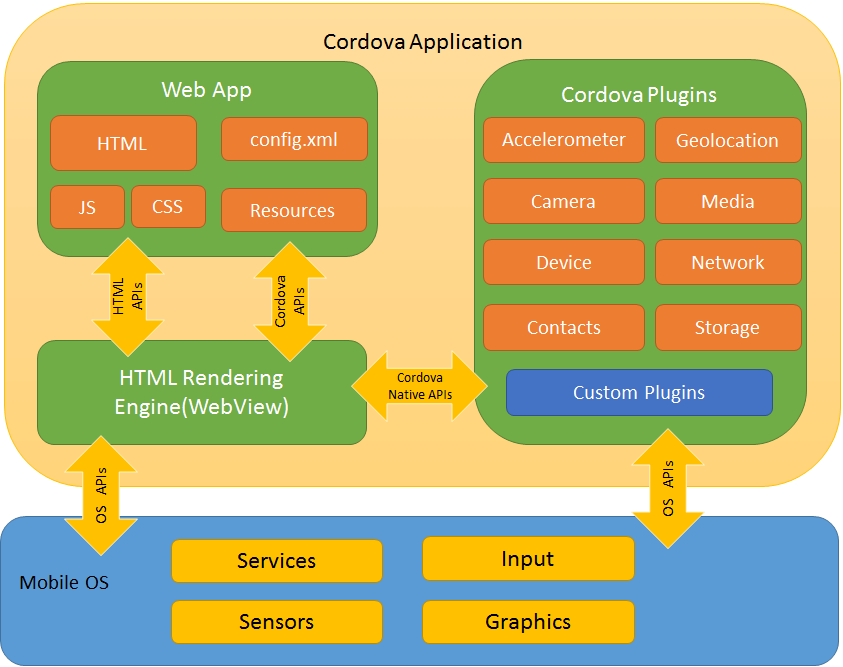
\includegraphics[width=0.75\linewidth]{chapter4/cordovaapparchitecture}
	    \caption{Arquitectura de Apache Cordova \cite{ACO}.}
	    \label{fig:ch05:cordova-arch}
    \end{center}
\end{figure}
\subsection{Aplicaciones Nativas vs Aplicaciones Híbridas}
Decimos que una aplicación es nativa cuando fue desarrollada específicamente para un sistema operativo móvil (Objective-C o Swift para iOS, Java para Android).\\

Dado que una aplicación nativa se desarrolla siguiendo las recomendaciones técnicas del sistema operativo, no solo tiene la ventaja de tener un rendimiento más rápido sino que también es más amigable, ya que tiene una apariencia similar a la mayoría de las otras aplicaciones nativas del dispositivo. Además, pueden acceder y utilizar fácilmente las capacidades integradas del dispositivo del usuario.\\

Por otra parte, decimos que una aplicación es híbrida cuando está basada en la web, construida principalmente con HTML5 y JavaScript, que luego se ejecuta en un \emph{contenedor} que proporciona acceso a las características de la plataforma nativa.\\

Las aplicaciones híbridas se ven como una aplicación nativa, pero, fuera del marco básico de la aplicación, sus contenidos son provistos por un servidor externo. Cuando el usuario instala una aplicación híbrida, se descargan la mayor parte del contenido. Posteriormente, mientras el usuario navega por la aplicación, se van descargando el resto de los contenidos según se vayan necesitando. Entre sus ventajas principales se encuentran que: dispone de todos los \emph{frameworks} disponibles para lenguajes web, el desarrollo es muliplataforma, y se programa en un solo lenguaje.
\subsection{Plugins}
Los \emph{Plugins} son una parte esencial dentro del ecosistema de Apache Cordova. Cada uno de ellos es un paquete de código inyectado que permite que la aplicación móvil se comunique con la plataforma nativa en la que se ejecuta. Los \emph{plugins} brindan acceso a funcionalidades del dispositivo y de la plataforma que normalmente no están disponibles para las aplicaciones basadas en la web \cite{ACP}.\\

Para hacer efectivo el mencionado acceso, los \emph{plugins} exponen una única interfaz de JavaScript. Apache Cordova realiza el enlace entre la interfaz Javascript y las correspondientes bibliotecas de códigos nativos, las cuales son provistas por el mismo \emph{plugin}. En esencia, un \emph{plugin} oculta las diversas implementaciones de código nativo detrás de una interfaz de JavaScript común.\\

Por otra parte, podemos clasificar a los \emph{plugins} en dos grandes grupos: \emph{Core Plugins} y \emph{Plugins Personalizados}. Los primeros proporcionan acceso a las funcionalidades básicas del dispositivo, tales como la batería, la cámara, los contactos, entre otros. Apache Cordova es el responsable de mantenerlos. Mientras que los segundos, son desarrollados por terceros y proporcionan accesos adicionales a funciones que no están necesariamente disponibles en todas las plataformas. El autor de dicho \emph{plugin} es responsable mantenerlo y de documentar cuáles plataformas soporta. Apache Cordova proporciona un buscador de \emph{plugins} o también se pueden descargar por \texttt{npm}.\\

Al crear un proyecto en Apache Cordova, por defecto no tiene \emph{plugins} instalados. Si se desean algún \emph{plugin}, inclusive los \emph{Core Plugins}, deben ser agregados explícitamente.